
%%%%%%%%%%%%%%%%%%%%%%% file typeinst.tex %%%%%%%%%%%%%%%%%%%%%%%%%
%
% This is the LaTeX source for the instructions to authors using
% the LaTeX document class 'llncs.cls' for contributions to
% the Lecture Notes in Computer Sciences series.
% http://www.springer.com/lncs       Springer Heidelberg 2006/05/04
%
% It may be used as a template for your own input - copy it
% to a new file with a new name and use it as the basis
% for your article.
%
% NB: the document class 'llncs' has its own and detailed documentation, see
% ftp://ftp.springer.de/data/pubftp/pub/tex/latex/llncs/latex2e/llncsdoc.pdf
%
%%%%%%%%%%%%%%%%%%%%%%%%%%%%%%%%%%%%%%%%%%%%%%%%%%%%%%%%%%%%%%%%%%%


\documentclass[runningheads,a4paper]{llncs2e/llncs}

\usepackage[T1]{fontenc}

\usepackage{amssymb,amsmath,bbm}
\setcounter{tocdepth}{3}
\usepackage{graphicx}

\usepackage{url}
\urldef{\mailjr}\path|juste.raimbault@polytechnique.edu|

  
\newcommand{\keywords}[1]{\par\addvspace\baselineskip
\noindent\keywordname\enspace\ignorespaces#1}

\newcommand{\noun}[1]{\textsc{#1}}

\usepackage[normalem]{ulem} % use normalem to protect \emph
\usepackage{xcolor}
\newcommand\change{\bgroup\markoverwith
  {\textcolor{yellow}{\rule[-.5ex]{2pt}{2.5ex}}}\ULon}




\begin{document}

\mainmatter  % start of an individual contribution




% first the title is needed
\title{Reconciling complexities: for a stronger integration of approaches to complex socio-technical systems}

% a short form should be given in case it is too long for the running head
\titlerunning{Reconciling complexities}

% the name(s) of the author(s) follow(s) next
%
% NB: Chinese authors should write their first names(s) in front of
% their surnames. This ensures that the names appear correctly in
% the running heads and the author index.
%
\author{\noun{Juste Raimbault}$^{1,2}$}
%
\authorrunning{Reconciling complexities}
% (feature abused for this document to repeat the title also on left hand pages)

% the affiliations are given next; don't give your e-mail address
% unless you accept that it will be published
\institute{$^{1}$ UMR CNRS 8504 G{\'e}ographie-Cit{\'e}s, Paris, France\\
$^{2}$ UMR-T IFSTTAR 9403 LVMT, Champs-sur-Marne, France\\
\mailjr
}

\toctitle{Lecture Notes in Computer Science}
\tocauthor{Authors' Instructions}
\maketitle


\begin{abstract}
System engineering has developed a mature knowledge on how to design, integrate and manage complex industrial systems, whereas disciplines studying complex systems in nature or society also propose numerous tools for their understanding. Socio-technical systems, that situate at their intersection, could benefit from a higher integration between these. This position paper advocates for such integrated approaches. A bibliometric study through citation networks first illustrates the respective isolation of some of these approaches. We then produce a proof-of-concept of how the transfer of concepts from biology can be useful for the design of complex systems, in the particular case of transportation networks, using a biological network growth model to produce various optimal networks in terms of cost and efficiency. We finally discuss possible disciplinary positioning of such hybrid approaches.
\keywords{System Engineering; Complex Systems Science; Bibliometrics; Bio-inspired Network Design; Integrative Disciplines}
\end{abstract}



%%%%%%%%%%%%%%%%
\section{Introduction}
%%%%%%%%%%%%%%%%


% - different types of complexities : systems engineering / even within complex systems
% - but finally treat of the same objects ? debates of top-down/bottom-up


\cite{chu2008criteria} recalls that several approaches to complexity do not

\cite{deffuant2015visions} actualize the metaphor of the Laplace Deamon, and develops three visions of complexity with progressive epistemological assumptions on the role of emergence.


\cite{ottino2004engineering} advocates for a stronger consideration of emerging properties in the engineering of complex systems, and claims for example that engineers and social scientists have much to exchange.


\cite{jennings2003agent} suggests that agent-based systems are an interesting alternative for the design of control systems, in particular thanks to their increased flexibility and robustness.

These issues of integrating complexities is indeed not particular to system engineering, as \cite{farmer2009economy} show that in the case of economics, policy-related benefits would be obtained by a more frequent use of agent-based approaches. 



The rest of the paper is organized as follows: we first develop a bibliometric study, in order to illustrate through the exploration of citation networks the effective separation of some branches of system engineerings and of complex systems science. We then develop a modeling case study to give a proof-of-study of how complex systems concepts, in this case from biology, can be used for the design of systems.



%%%%%%%%%%%%%%%%
\section{A bibliometric insight}
%%%%%%%%%%%%%%%%

\subsection{Context}

Statements about disciplines, their positioning and their relations, must often be taken with caution, including ours, as they will depend on the perspective taken to enter the problem, on the information available, on possible higher contexts implying sociological issues \cite{latour1977rhetorique}. They furthermore involve issues of reflexivity if they are done by researchers in the field themselves, implying to find what Morin calls a ``meta-viewpoint'' to construct an integrated knowledge \cite{edgar1986methode}. However, a growing body of knowledge in bibliometrics, that can be understood as a \emph{quantitative epistemology} \cite{chavalarias2013phylomemetic}

\cite{waltman2010unified}

\subsection{Method}

We use here the tool provided by \cite{raimbault2017exploration} to reconstruct backward citation networks

% criteria : survey ; enough citations.

\cite{estefan2007survey} as the origin node for system engineerings
% Incose

\cite{newman2011complex} for complex systems
% not too specialized, as network science ; agent-based ; dynamical systems ; etc.
% -> good compromise ?


\subsection{Results}



% recall limitation : not latest reference for example



%%% Corpus
% Survey of model-based systems engineering (MBSE) methodologies;5581471115472258458
%  2nd order neigh :
%.  3037/4019 vertices
%. Modularity: 0.716

% Complex systems: A survey;4678769739448217155
%  2nd order neigh : 1304/4019 vertices
% Modularity: 0.799
%
% intersection(incid1,incid2)
% + 2/4019 vertices


%%% Results

% ecount(citationcore)/(vcount(citationcore)*(vcount(citationcore)-1))
% 0.002701705

%mean(degree(citation))
% 2.444887

%mean(degree(citation,mode = 'in'))
% 1.222443

%mean(degree(citationcore,mode = 'in'))
% 2.131646

% directedmodularity(com$membership,A)
%[1] 0.5855703

%show(paste0(mean(mods)," +- ",sd(mods)))
% [1] "-0.000427444129744247 +- 0.00601916650457223



%%%%%%%%%%%%%%
\begin{figure}
	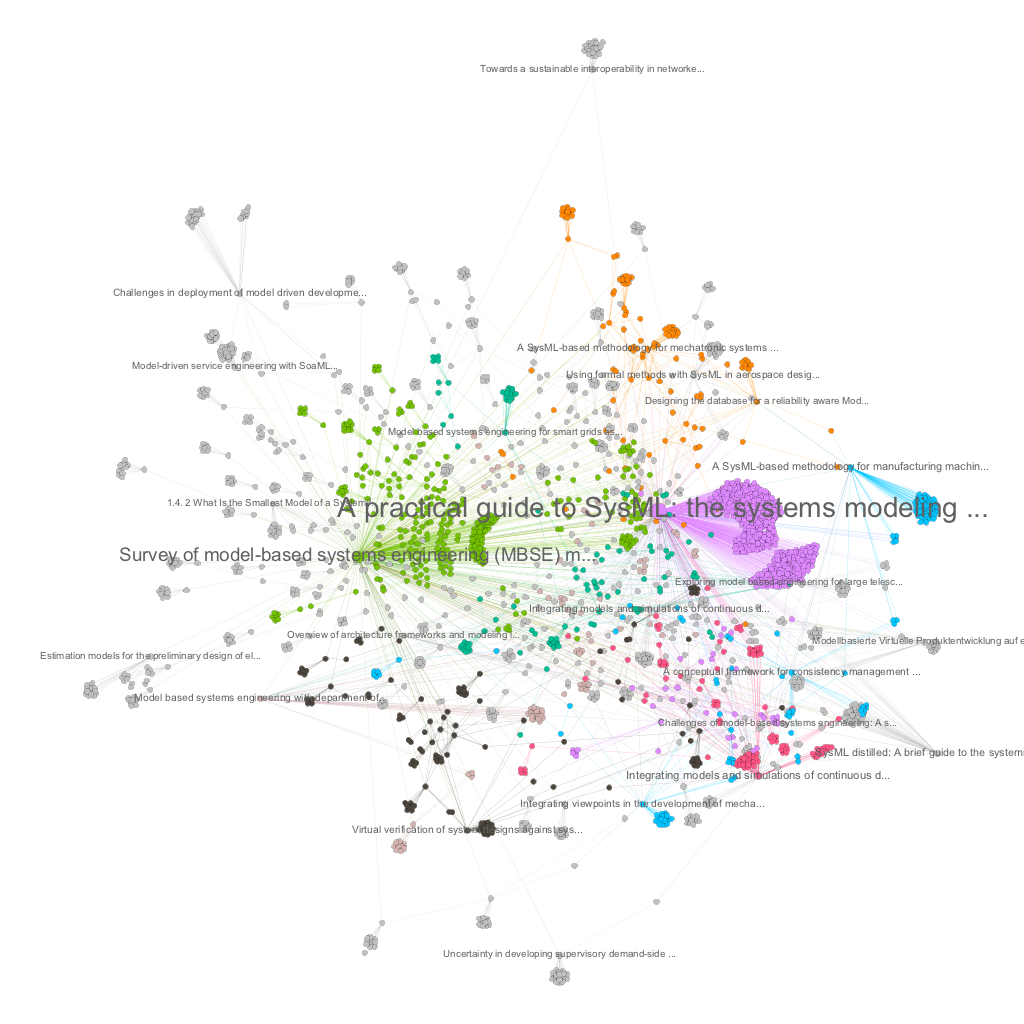
\includegraphics[width=\linewidth,height=0.6\textheight]{figures/cseng.png}\\
	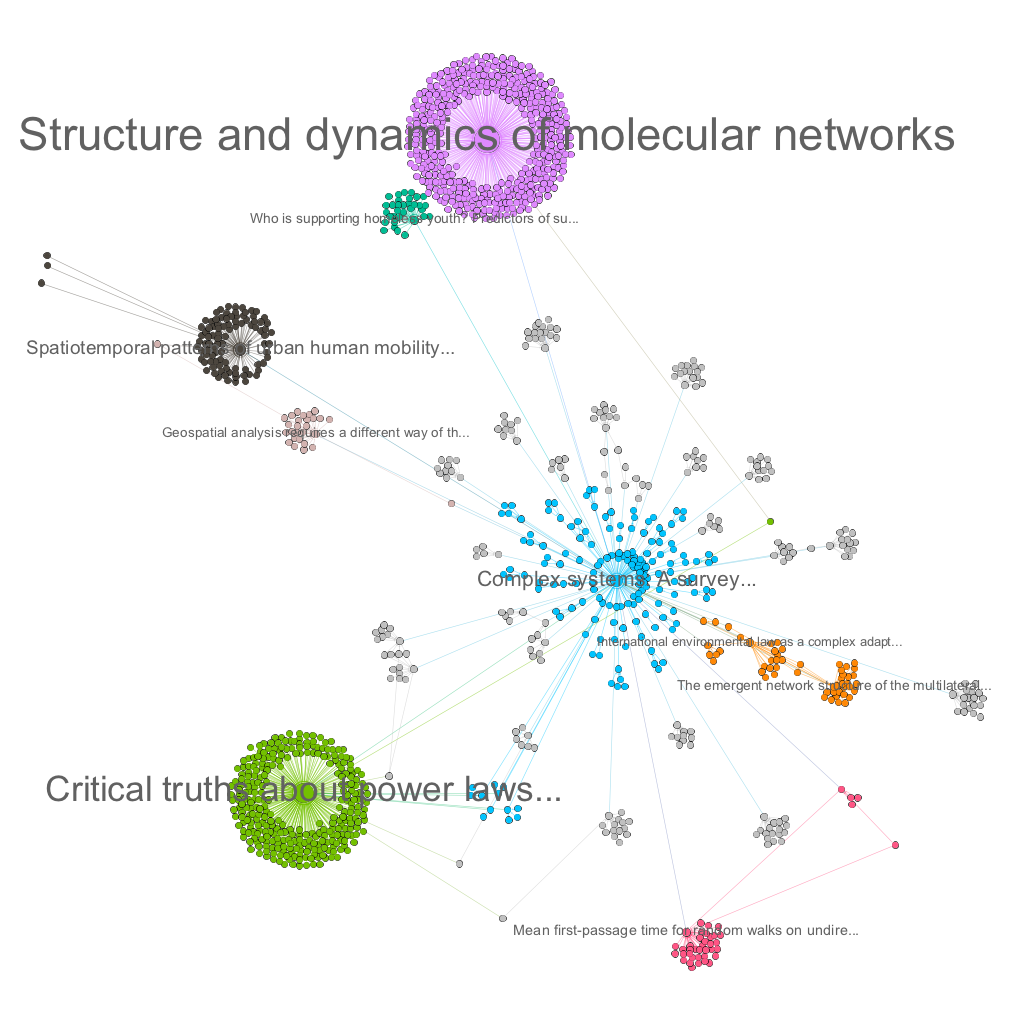
\includegraphics[width=\linewidth,height=0.6\textheight]{figures/csnatural.png}
	\caption{\textbf{Citation networks for each field.} \textit{(Top)} Citation network for the sample corresponding to system engineering approaches; \textit{(Bottom)} Citation network for the sample corresponding to complex systems science approaches.\label{fig:bothcitnw}}
\end{figure}
%%%%%%%%%%%%%%


%%%%%%%%%%%%%%
\begin{figure}
	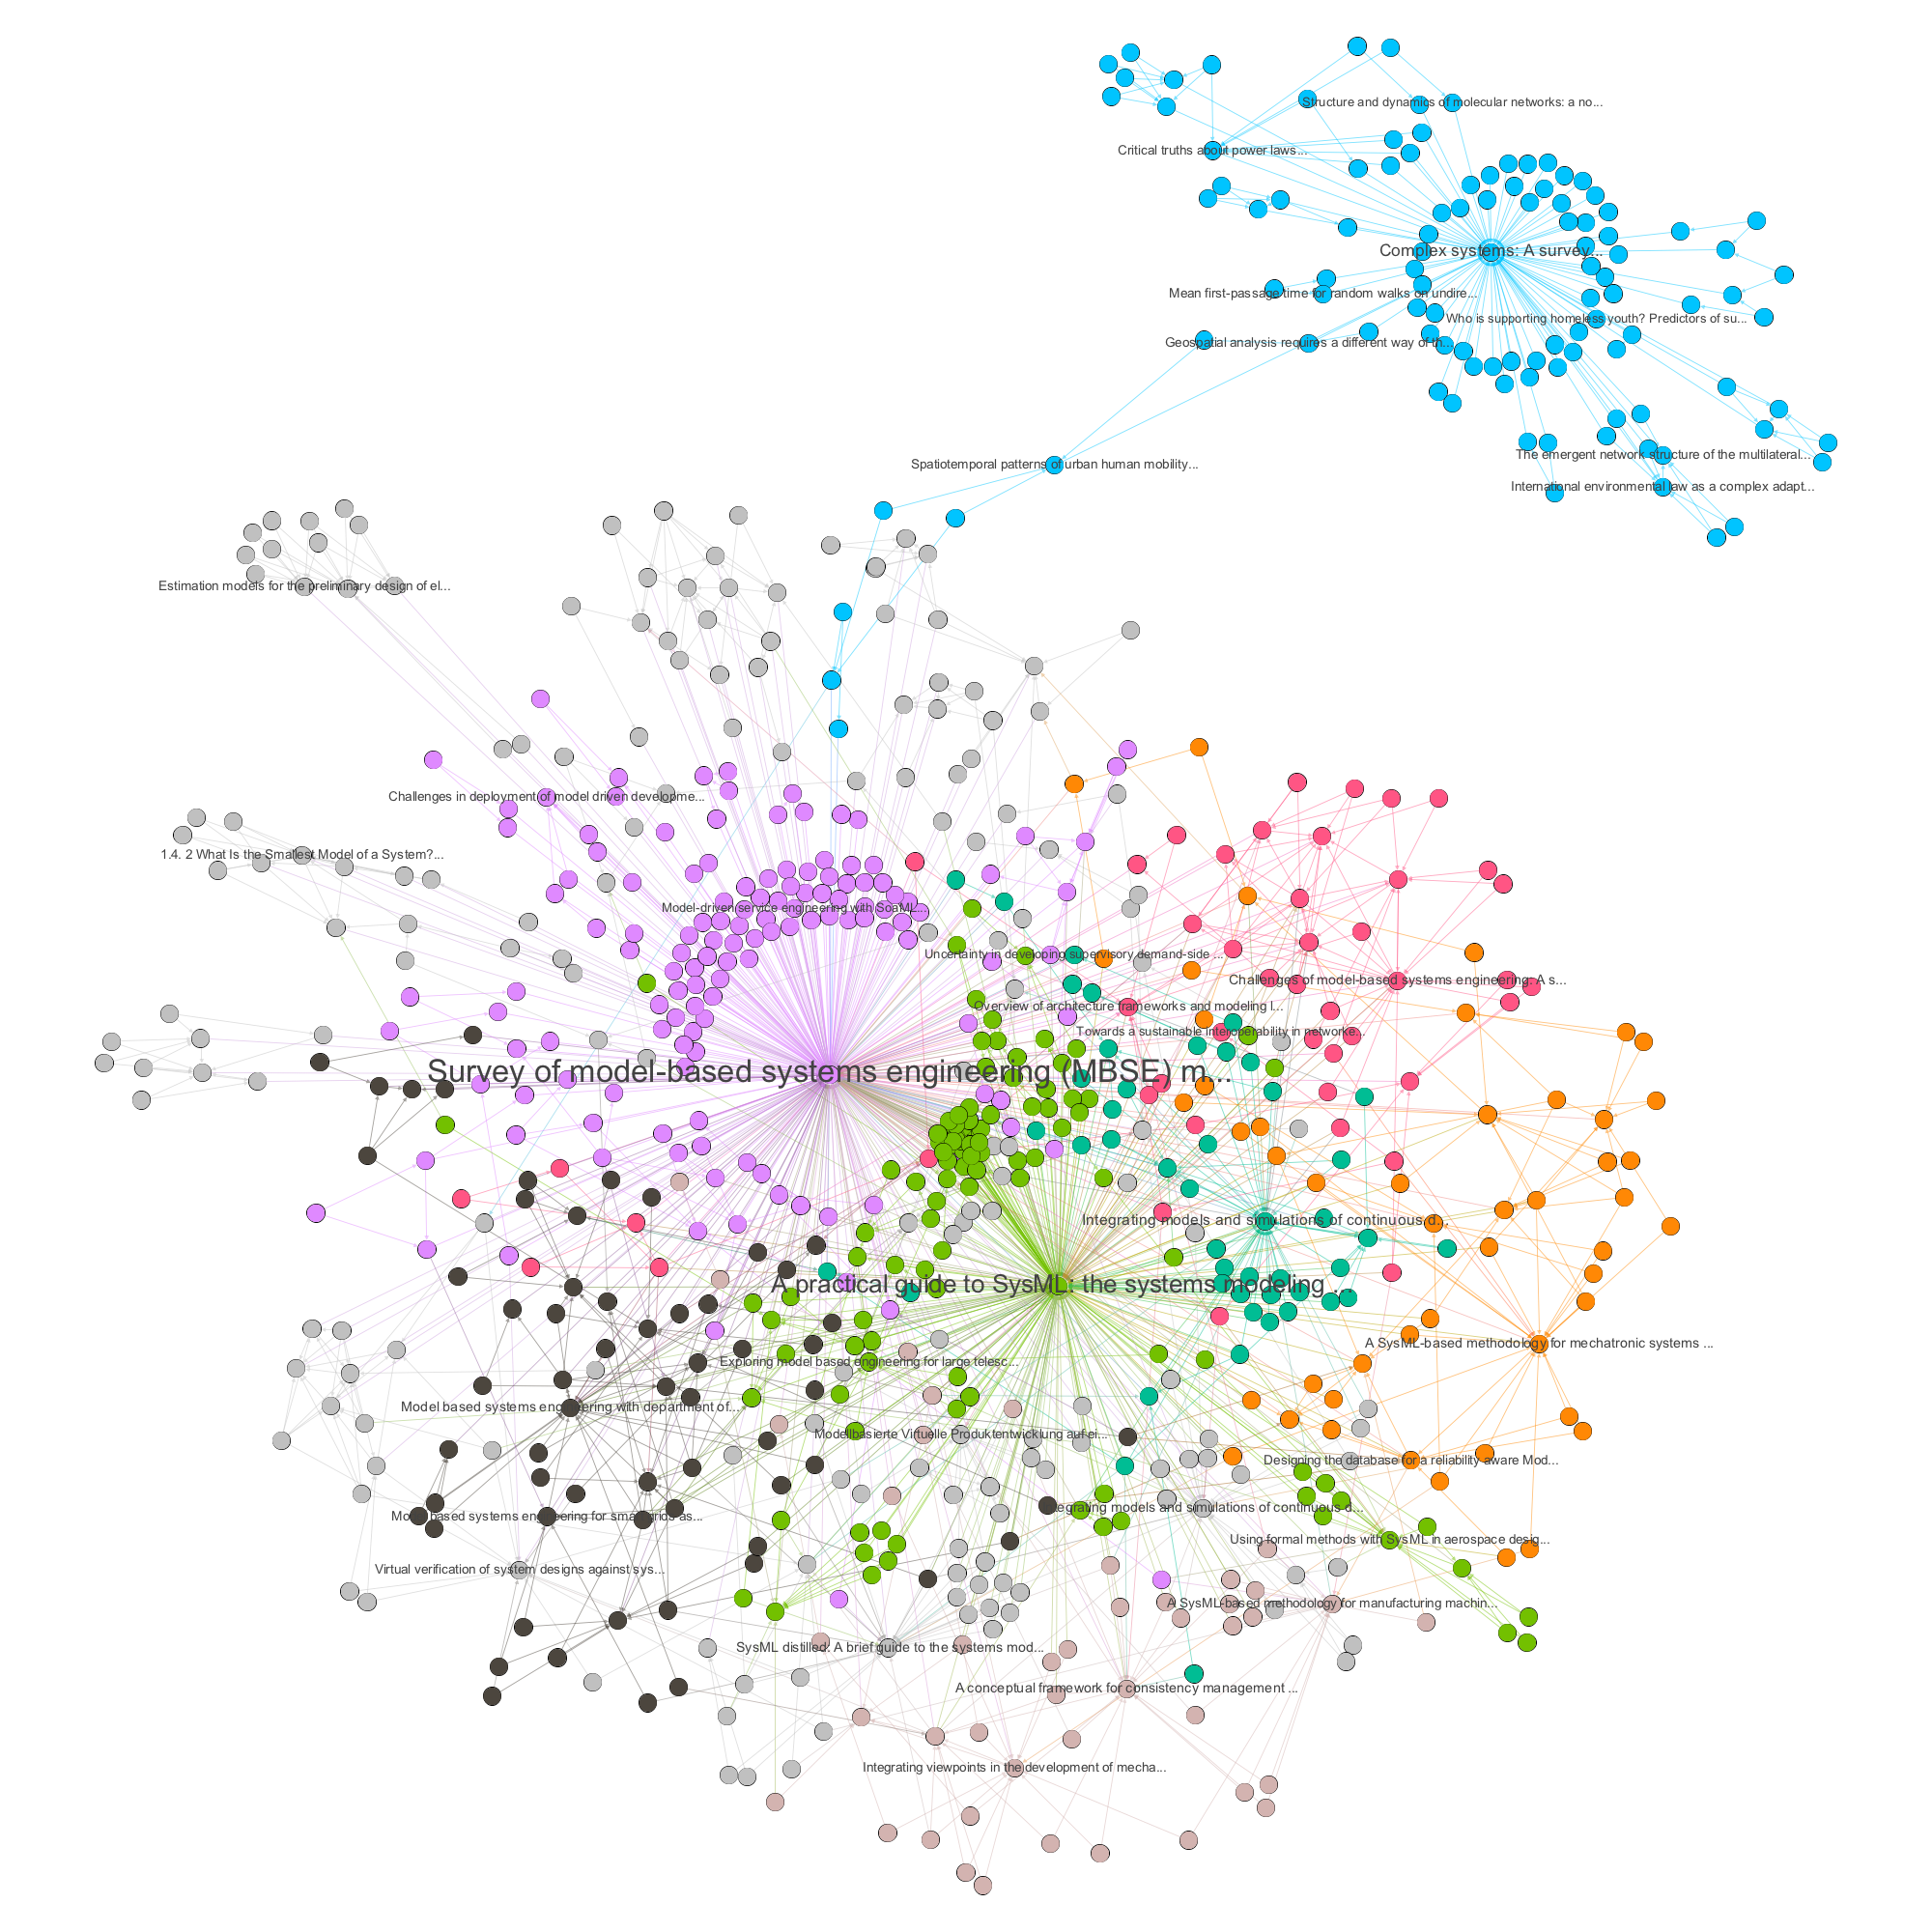
\includegraphics[width=\linewidth]{figures/core.png}
	\caption{\textbf{Full citation network.} We show the core of the full citation network, corresponding to nodes with a degree larger than one and corresponding edges, to ease readability. The two components shown in Fig.~\ref{fig:bothcitnw} are connected by a small bridge only.\label{fig:citnw}}
\end{figure}
%%%%%%%%%%%%%%





%%%%%%%%%%%%%%%%
\section{A proof-of-concept: biological network generation}
%%%%%%%%%%%%%%%%


\subsection{Context}

How can the transfer of concepts from other disciplines can inform system design ? Contributions giving elements of answer to this question are indeed not new, and the entire field of \emph{Artificial Life} 



\cite{beer2004autopoiesis} autopoiesis and cognition in the game of life


\subsection{Network generation model}


We detail here the model of type \emph{slime mould} used to evolve a biological network, introduced by~\cite{tero2007mathematical}. The network is composed by nodes characterized by their pressure $p_i$ and by links characterized by their length $L_{ij}$, their diameter $D_{ij}$, an impedance $Z_{ij}$ and the flow traversing them $\phi_{ij}$. The topology of the network is assumed fixed, but the diameters of links can evolve in time.


The flows are characterized by a relation analogous to Ohm's law on links which writes

\[
\phi_{ij} = \frac{D_{ij}}{Z_{ij}\cdot L_{ij}} \left(p_i - p_j\right)
\]

Furthermore, the conservation of flows at each node (Kirchoff's law) imposes

\[
\sum_i \phi_{ij} = 0
\]

for all $j$ except the source and the sink, that we assume at indices $j_+$ and $j_-$, such that $\sum_i \phi_{ij_+} = I_0$ and $\sum_i \phi_{ij_-} = -I_0$ with $I_0$ initial flow parameter.

The combination of above constraints gives for all $j$

\[
\sum_i \frac{D_{ij}}{Z_{ij}\cdot L_{ij}} (p_i - p_j) = \mathbbm{1}_{j=j_+} I_0 - \mathbbm{1}_{j=j_-} I_0 
\]

what simplifies into a matrix equation, by denoting $\mathbf{Z} = \left(\frac{\frac{D_{ij}}{Z_{ij}\cdot L_{ij}}}{\sum_i \frac{D_{ij}}{Z_{ij}\cdot L_{ij}}}\right)_{ij}$, and also $\vec{k} = \frac{\mathbbm{1}_{j=j_+} I_0 - \mathbbm{1}_{j=j_-} I_0 }{\sum_i \frac{D_{ij}}{Z_{ij}\cdot L_{ij}}}$ and $\vec{p} = p_i$, what simplifies into

\[
\left(Id - \mathbf{Z}\right) \vec{p} = \vec{k}
\]

The system admits a solution when $\left(Id - \mathbf{Z}\right)$ is invertible. The space of invertible matrices being dense in $\mathcal{M}_n(\mathbb{R})$, by multilinearity of the determinant, an infinitesimal perturbation of the position of nodes allows to invert the matrix if it is indeed singular. We obtain thus the pressures $p_i$ and as a consequence the flows $\phi_{ij}$.

The evolution of the diameter $D_{ij}$ between two equilibrium stages is a function of the flow at equilibrium, through the equation


\[
D_{ij} (t+1) - D_{ij} = \delta t \left[ \frac{\phi_{ij}(t)^\gamma}{1 + \phi_{ij}(t)^\gamma} - D_{ij}(t)\right]
\]

We take to simplify $\gamma = 1.8$, following the configuration used by~\cite{tero2010rules} for the generation of a network in a real configuration. We furthermore take $\delta t = 0.05$ and $I_0 = 10$.


The generation of a network can be achieved from an initial network, until reaching a convergence criteria, for example $\sum_{ij} \Delta D_{ij} (t) < \varepsilon$ with $\varepsilon$ fixed threshold parameter. We will use this model with a criteria of a number of iterations, and proceed to an iteration to obtain final networks with a reasonable number of links.




%%%%%%%%%%%%%%%%%%
\subsection{Results}


\subsubsection{Designing public transportation lines}



%%%%%%%%%%%%%
\begin{figure}
	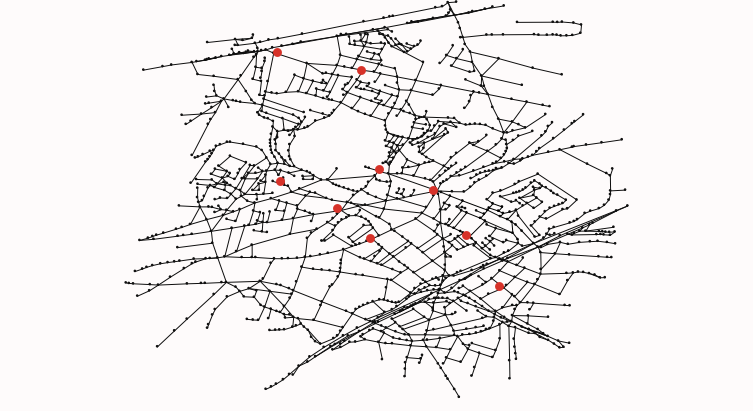
\includegraphics[width=0.32\textwidth]{figures/slimemould_tick1.png}
	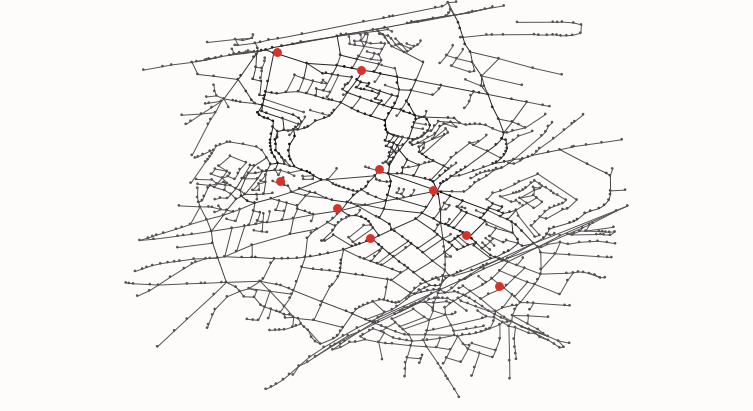
\includegraphics[width=0.32\textwidth]{figures/slimemould_tick10.png}
	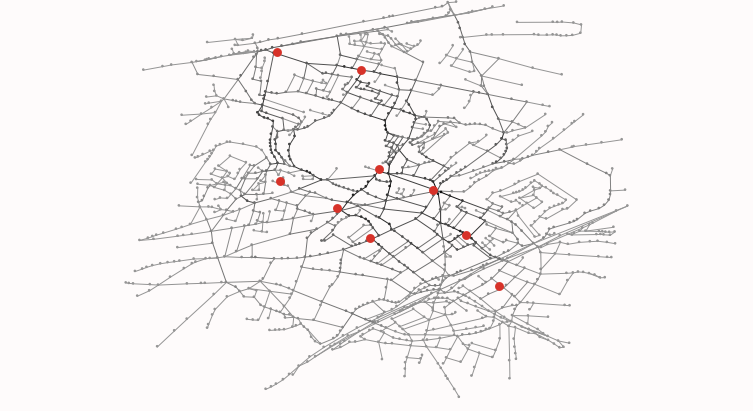
\includegraphics[width=0.32\textwidth]{figures/slimemould_tick20.png}\\
	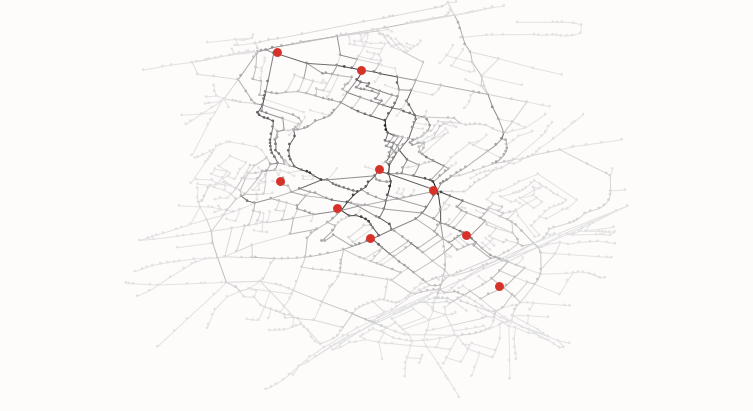
\includegraphics[width=0.32\textwidth]{figures/slimemould_tick50.png}
	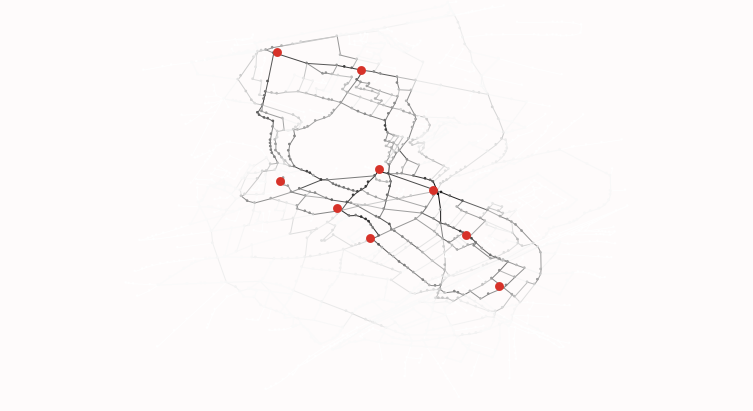
\includegraphics[width=0.32\textwidth]{figures/slimemould_tick101.png}
	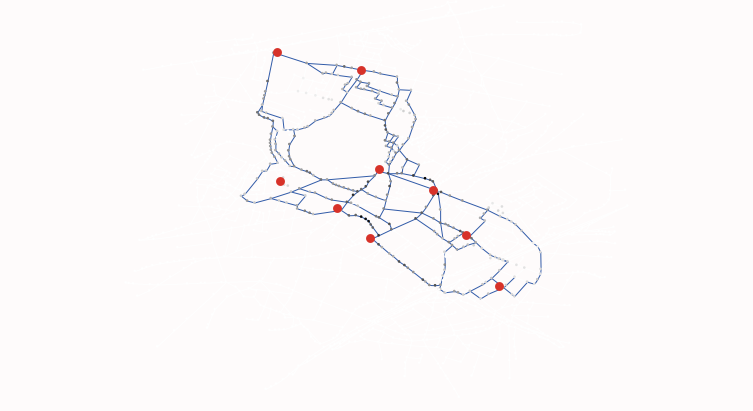
\includegraphics[width=0.32\textwidth]{figures/slimemould_reseauFinal.png}
	\caption{\textbf{Application of the slime mould model to design a robust public transportation network.}\label{fig:romainville}}
\end{figure}
%%%%%%%%%%%%%



\subsubsection{Generating optimal networks}




%%%%%%%%%%%%%%
\begin{figure}
	
	\caption{Example of networks.}
\end{figure}
%%%%%%%%%%%%%%




%%%%%%%%%%%%%%
\begin{figure}
	
	\caption{Optimality of simulated networks.}
\end{figure}
%%%%%%%%%%%%%%




%%%%%%%%%%%%%%%%
\section{Discussion}
%%%%%%%%%%%%%%%%

%. -> roadmap / towards integrated disciplines ? (add knowledge domains integration ?)
%  -> morphogenetic engineering as an example of such a discipline



%%%%%%%%%%%%%%%%
\section{Conclusion}
%%%%%%%%%%%%%%%%






\section*{Acknowledgments}

% EGI


%%%%%%%%%%%%%%%%
%% Biblio
%%%%%%%%%%%%%%%%


\bibliographystyle{unsrt}
\bibliography{biblio}
%\bibliography{biblio/biblio,/Users/Juste/Documents/ComplexSystems/CityNetwork/Biblio/BibTeX/CityNetwork}






\end{document}
